% GNUPLOT: LaTeX picture with Postscript
\begingroup
  \makeatletter
  \providecommand\color[2][]{%
    \GenericError{(gnuplot) \space\space\space\@spaces}{%
      Package color not loaded in conjunction with
      terminal option `colourtext'%
    }{See the gnuplot documentation for explanation.%
    }{Either use 'blacktext' in gnuplot or load the package
      color.sty in LaTeX.}%
    \renewcommand\color[2][]{}%
  }%
  \providecommand\includegraphics[2][]{%
    \GenericError{(gnuplot) \space\space\space\@spaces}{%
      Package graphicx or graphics not loaded%
    }{See the gnuplot documentation for explanation.%
    }{The gnuplot epslatex terminal needs graphicx.sty or graphics.sty.}%
    \renewcommand\includegraphics[2][]{}%
  }%
  \providecommand\rotatebox[2]{#2}%
  \@ifundefined{ifGPcolor}{%
    \newif\ifGPcolor
    \GPcolorfalse
  }{}%
  \@ifundefined{ifGPblacktext}{%
    \newif\ifGPblacktext
    \GPblacktexttrue
  }{}%
  % define a \g@addto@macro without @ in the name:
  \let\gplgaddtomacro\g@addto@macro
  % define empty templates for all commands taking text:
  \gdef\gplbacktext{}%
  \gdef\gplfronttext{}%
  \makeatother
  \ifGPblacktext
    % no textcolor at all
    \def\colorrgb#1{}%
    \def\colorgray#1{}%
  \else
    % gray or color?
    \ifGPcolor
      \def\colorrgb#1{\color[rgb]{#1}}%
      \def\colorgray#1{\color[gray]{#1}}%
      \expandafter\def\csname LTw\endcsname{\color{white}}%
      \expandafter\def\csname LTb\endcsname{\color{black}}%
      \expandafter\def\csname LTa\endcsname{\color{black}}%
      \expandafter\def\csname LT0\endcsname{\color[rgb]{1,0,0}}%
      \expandafter\def\csname LT1\endcsname{\color[rgb]{0,1,0}}%
      \expandafter\def\csname LT2\endcsname{\color[rgb]{0,0,1}}%
      \expandafter\def\csname LT3\endcsname{\color[rgb]{1,0,1}}%
      \expandafter\def\csname LT4\endcsname{\color[rgb]{0,1,1}}%
      \expandafter\def\csname LT5\endcsname{\color[rgb]{1,1,0}}%
      \expandafter\def\csname LT6\endcsname{\color[rgb]{0,0,0}}%
      \expandafter\def\csname LT7\endcsname{\color[rgb]{1,0.3,0}}%
      \expandafter\def\csname LT8\endcsname{\color[rgb]{0.5,0.5,0.5}}%
    \else
      % gray
      \def\colorrgb#1{\color{black}}%
      \def\colorgray#1{\color[gray]{#1}}%
      \expandafter\def\csname LTw\endcsname{\color{white}}%
      \expandafter\def\csname LTb\endcsname{\color{black}}%
      \expandafter\def\csname LTa\endcsname{\color{black}}%
      \expandafter\def\csname LT0\endcsname{\color{black}}%
      \expandafter\def\csname LT1\endcsname{\color{black}}%
      \expandafter\def\csname LT2\endcsname{\color{black}}%
      \expandafter\def\csname LT3\endcsname{\color{black}}%
      \expandafter\def\csname LT4\endcsname{\color{black}}%
      \expandafter\def\csname LT5\endcsname{\color{black}}%
      \expandafter\def\csname LT6\endcsname{\color{black}}%
      \expandafter\def\csname LT7\endcsname{\color{black}}%
      \expandafter\def\csname LT8\endcsname{\color{black}}%
    \fi
  \fi
    \setlength{\unitlength}{0.0500bp}%
    \ifx\gptboxheight\undefined%
      \newlength{\gptboxheight}%
      \newlength{\gptboxwidth}%
      \newsavebox{\gptboxtext}%
    \fi%
    \setlength{\fboxrule}{0.5pt}%
    \setlength{\fboxsep}{1pt}%
    \definecolor{tbcol}{rgb}{1,1,1}%
\begin{picture}(8640.00,7200.00)%
    \gplgaddtomacro\gplbacktext{%
      \csname LTb\endcsname%%
      \put(4687,795){\makebox(0,0){\strut{}$20$}}%
      \csname LTb\endcsname%%
      \put(4283,948){\makebox(0,0){\strut{}$30$}}%
      \csname LTb\endcsname%%
      \put(3878,1101){\makebox(0,0){\strut{}$40$}}%
      \csname LTb\endcsname%%
      \put(3473,1254){\makebox(0,0){\strut{}$50$}}%
      \csname LTb\endcsname%%
      \put(3068,1407){\makebox(0,0){\strut{}$60$}}%
      \csname LTb\endcsname%%
      \put(2663,1561){\makebox(0,0){\strut{}$70$}}%
      \csname LTb\endcsname%%
      \put(2258,1714){\makebox(0,0){\strut{}$80$}}%
      \csname LTb\endcsname%%
      \put(1854,1867){\makebox(0,0){\strut{}$90$}}%
      \csname LTb\endcsname%%
      \put(1449,2020){\makebox(0,0){\strut{}$100$}}%
      \csname LTb\endcsname%%
      \put(1044,2173){\makebox(0,0){\strut{}$110$}}%
      \csname LTb\endcsname%%
      \put(7755,2646){\makebox(0,0){\strut{}$2.2$}}%
      \csname LTb\endcsname%%
      \put(7412,2417){\makebox(0,0){\strut{}$2.25$}}%
      \csname LTb\endcsname%%
      \put(7068,2189){\makebox(0,0){\strut{}$2.3$}}%
      \csname LTb\endcsname%%
      \put(6725,1960){\makebox(0,0){\strut{}$2.35$}}%
      \csname LTb\endcsname%%
      \put(6382,1732){\makebox(0,0){\strut{}$2.4$}}%
      \csname LTb\endcsname%%
      \put(6039,1503){\makebox(0,0){\strut{}$2.45$}}%
      \csname LTb\endcsname%%
      \put(5695,1275){\makebox(0,0){\strut{}$2.5$}}%
      \csname LTb\endcsname%%
      \put(5352,1046){\makebox(0,0){\strut{}$2.55$}}%
      \csname LTb\endcsname%%
      \put(5009,817){\makebox(0,0){\strut{}$2.6$}}%
      \put(999,2263){\makebox(0,0)[r]{\strut{}$2$}}%
      \put(999,2596){\makebox(0,0)[r]{\strut{}$3$}}%
      \put(999,2930){\makebox(0,0)[r]{\strut{}$4$}}%
      \put(999,3263){\makebox(0,0)[r]{\strut{}$5$}}%
      \put(999,3596){\makebox(0,0)[r]{\strut{}$6$}}%
      \put(999,3929){\makebox(0,0)[r]{\strut{}$7$}}%
      \put(999,4262){\makebox(0,0)[r]{\strut{}$8$}}%
      \put(999,4594){\makebox(0,0)[r]{\strut{}$9$}}%
      \put(999,4927){\makebox(0,0)[r]{\strut{}$10$}}%
      \put(999,5260){\makebox(0,0)[r]{\strut{}$11$}}%
      \put(999,5593){\makebox(0,0)[r]{\strut{}$12$}}%
      \put(999,5926){\makebox(0,0)[r]{\strut{}$13$}}%
    }%
    \gplgaddtomacro\gplfronttext{%
      \csname LTb\endcsname%%
      \put(7395,6307){\makebox(0,0)[r]{\strut{}$ I_v = 82.0 $ mA}}%
      \csname LTb\endcsname%%
      \put(7395,6087){\makebox(0,0)[r]{\strut{}$ I_v = 62.8 $ mA}}%
      \csname LTb\endcsname%%
      \put(7395,5867){\makebox(0,0)[r]{\strut{}$ U_a = 1750 $ V}}%
      \csname LTb\endcsname%%
      \put(7395,5647){\makebox(0,0)[r]{\strut{}$ U_a = 2000 $ V}}%
      \csname LTb\endcsname%%
      \put(2558,1315){\makebox(0,0){\strut{}$ I_v $ (mA)}}%
      \put(7847,1604){\makebox(0,0){\strut{}$ U_a^{-1/2} \cdot 10^{-2} $  $ (kV^{-1/2})  $ }}%
      \put(201,4095){\makebox(0,0){\strut{}$ y $ (cm)}}%
    }%
    \gplbacktext
    \put(0,0){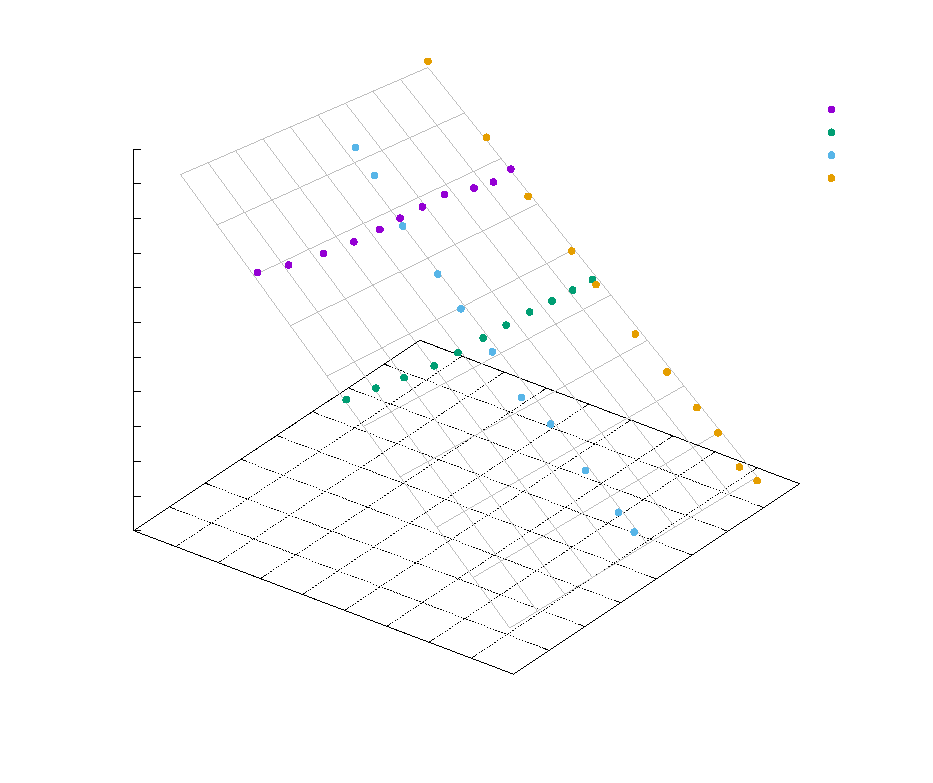
\includegraphics[width={432.00bp},height={360.00bp}]{3dvychylovani}}%
    \gplfronttext
  \end{picture}%
\endgroup
